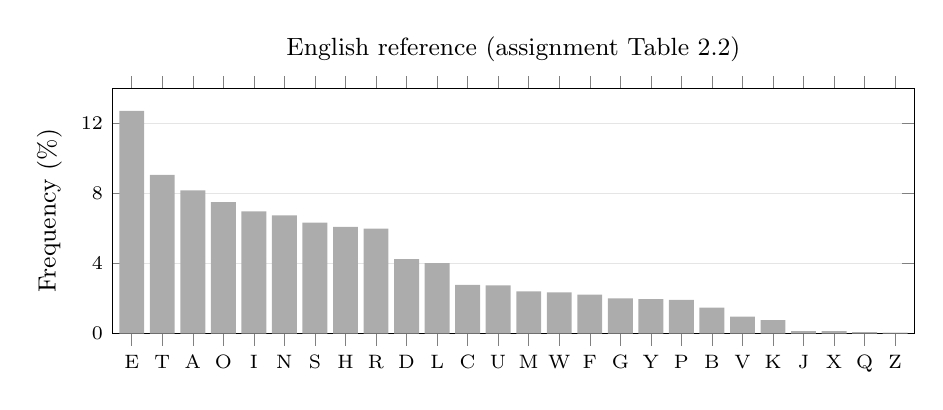
\begin{tikzpicture}
\begin{axis}[width=0.97\textwidth,height=4.7cm,ybar,bar width=9pt,ymin=0,ymax=14,ytick={0,4,8,12},ylabel={Frequency (\%)},symbolic x coords={E,T,A,O,I,N,S,H,R,D,L,C,U,M,W,F,G,Y,P,B,V,K,J,X,Q,Z},xtick=data,xticklabel style={font=\scriptsize},title={English reference (assignment Table 2.2)},title style={font=\small},tick label style={font=\scriptsize},label style={font=\small},ymajorgrids=true,grid style={gray!20},enlarge x limits=0.025]
\addplot[fill=gray!65,draw=none] coordinates {(E,12.7000) (T,9.0600) (A,8.1700) (O,7.5100) (I,6.9700) (N,6.7500) (S,6.3300) (H,6.0900) (R,5.9900) (D,4.2500) (L,4.0300) (C,2.7800) (U,2.7600) (M,2.4100) (W,2.3600) (F,2.2300) (G,2.0100) (Y,1.9700) (P,1.9300) (B,1.4900) (V,0.9800) (K,0.7700) (J,0.1500) (X,0.1500) (Q,0.0900) (Z,0.0700)};
\end{axis}
\end{tikzpicture}
\par\vspace{0.3cm}
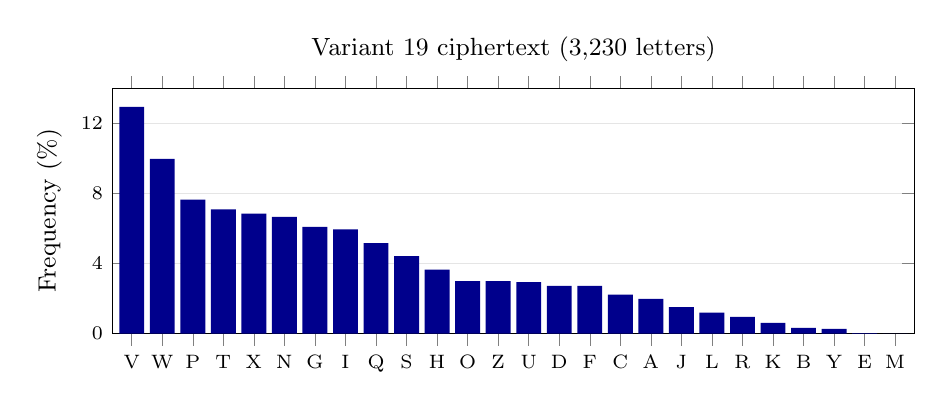
\begin{tikzpicture}
\begin{axis}[width=0.97\textwidth,height=4.7cm,ybar,bar width=9pt,ymin=0,ymax=14,ytick={0,4,8,12},ylabel={Frequency (\%)},symbolic x coords={V,W,P,T,X,N,G,I,Q,S,H,O,Z,U,D,F,C,A,J,L,R,K,B,Y,E,M},xtick=data,xticklabel style={font=\scriptsize},title={Variant 19 ciphertext (3,230 letters)},title style={font=\small},tick label style={font=\scriptsize},label style={font=\small},ymajorgrids=true,grid style={gray!20},enlarge x limits=0.025]
\addplot[fill=blue!55!black,draw=none] coordinates {(V,12.9412) (W,9.9690) (P,7.6471) (T,7.0898) (X,6.8421) (N,6.6563) (G,6.0991) (I,5.9443) (Q,5.1703) (S,4.4272) (H,3.6533) (O,3.0031) (Z,3.0031) (U,2.9412) (D,2.7245) (F,2.7245) (C,2.2291) (A,1.9814) (J,1.5170) (L,1.2074) (R,0.9598) (K,0.6192) (B,0.3406) (Y,0.2786) (E,0.0310) (M,0.0000)};
\end{axis}
\end{tikzpicture}
